\testfile{pgfplotstest.errorbars.tex}
\testsection{Errorbars}
{
\pgfplotstableread{plotdata/pgfplotstest_plot}\TABLEMACRO

%\tracingmacros=2\tracingcommands=2
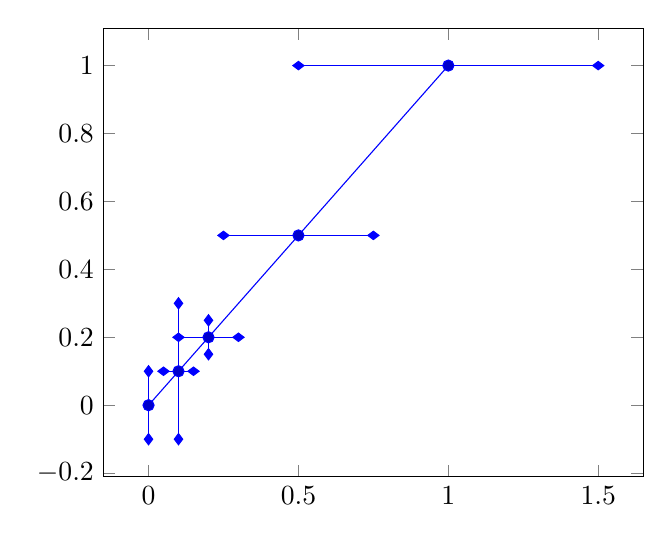
\begin{tikzpicture}
\begin{axis}
\addplot plot[
	error bars/.cd,
	y dir=both,y explicit,
	x dir=both,x fixed relative=0.5,
	error mark=diamond*,
]
	coordinates
	{(0,0) +- (0.5,0.1) 
	(0.1,0.1)  +- (0.05,0.2)
	(0.2,0.2) 	+- (0,0.05)
	(0.5,0.5)
	(1,1)};
\end{axis}
\end{tikzpicture}

\testsubsubsection{changing styles}
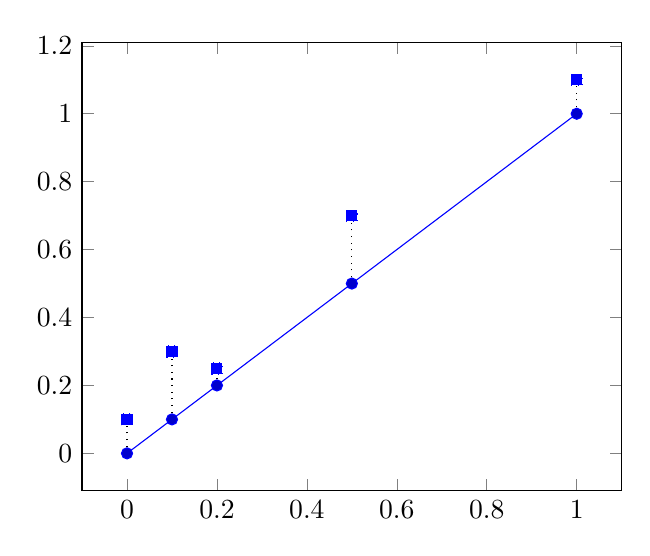
\begin{tikzpicture}
\begin{axis}
\addplot plot[
	error bars/.cd,
	y dir=plus,y explicit,
	error bar style={black,dotted,error bars/error mark=square*,error bars/error mark options={current plot style}},
]
	coordinates
	{(0,0) +- (0.5,0.1) 
	(0.1,0.1)  +- (0.05,0.2)
	(0.2,0.2) 	+- (0,0.05)
	(0.5,0.5) +- (0.1,0.2)
	(1,1) +- (0.3,0.1)
	};
\end{axis}
\end{tikzpicture}

\testsubsubsection{using 100\% minus}
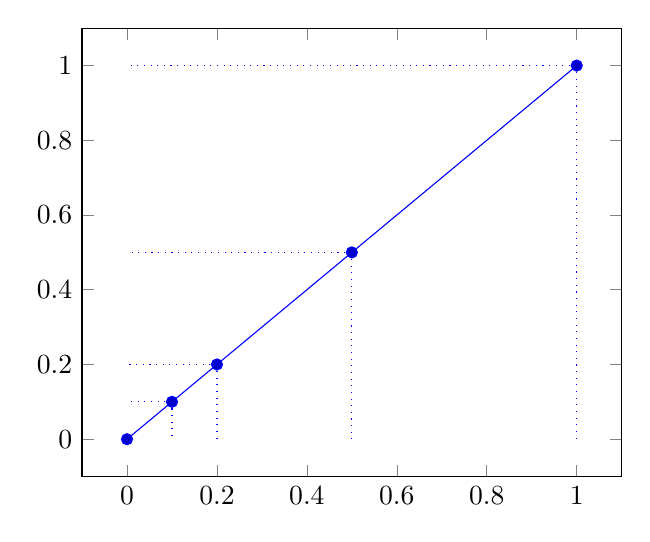
\begin{tikzpicture}
\begin{axis}
\addplot plot[
	error bars/.cd,
	y dir=minus,y fixed relative=1,
	x dir=minus,x fixed relative=1,
	error mark=none,
	error bar style={dotted},
]
	coordinates
	{(0,0) 
	(0.1,0.1)  
	(0.2,0.2) 	
	(0.5,0.5) 
	(1,1) 
	};
\end{axis}
\end{tikzpicture}
%
\testsubsubsection{with plot table}
\begin{sidewaystable}
{%
\lstset{
	showtabs=true,
	showspaces=true,
	basicstyle=\footnotesize\ttfamily,
	numbers=left,
	numberblanklines=true,
	breaklines=false,
	tabsize=15}
\lstinputlisting{plotdata/pgfplotstest_plot}
}
\caption{The table used for the plot table tests and error bars.}
\label{tbl:k}
\end{sidewaystable}

\begin{tikzpicture}
\begin{axis}[
	tick align=outside,
	grid=both,
	title={maxlevel versus cgiter, table~\ref{tbl:k}}]
\addplot plot[
	error bars/.cd,
	y dir=both,y explicit,
] table[x=maxlevel,y=cgiter,y error=cgiter_err] {plotdata/pgfplotstest_plot};

\end{axis}
\end{tikzpicture}

\testsubsubsection{with plot table from macro}
\begin{tikzpicture}
\begin{axis}[
	tick align=outside,
	grid=both,
	title={maxlevel versus cgiter, table~\ref{tbl:k}}]
\addplot plot[
	error bars/.cd,
	y dir=both,y explicit,
] table[x=maxlevel,y=cgiter,y error=cgiter_err] from \TABLEMACRO;

\end{axis}
\end{tikzpicture}

\testsubsection{Log-plot}
\testsubsubsection{relative errors}
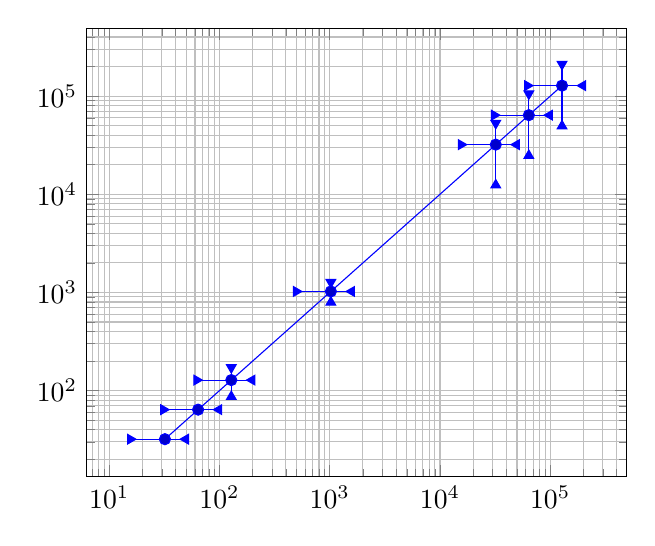
\begin{tikzpicture}
\begin{loglogaxis}[
	grid=both]
\addplot plot[
	error bars/.cd,
	y dir=both,y explicit relative,
	x dir=both,x fixed relative=0.5,
	error mark=triangle*,
]
	coordinates {
		(32,32)
		(64,64)
		(128,128) +- (0,0.3)
		(1024,1024) +- (0,0.2)
		(32068,32068)  +- (0,0.6)
		(64000,64000) +- (0,0.6)
		(128000,128000) +- (0,0.6)
	};

\end{loglogaxis}
\end{tikzpicture}

\testsubsubsection{x fixed=500, y explicit relative}
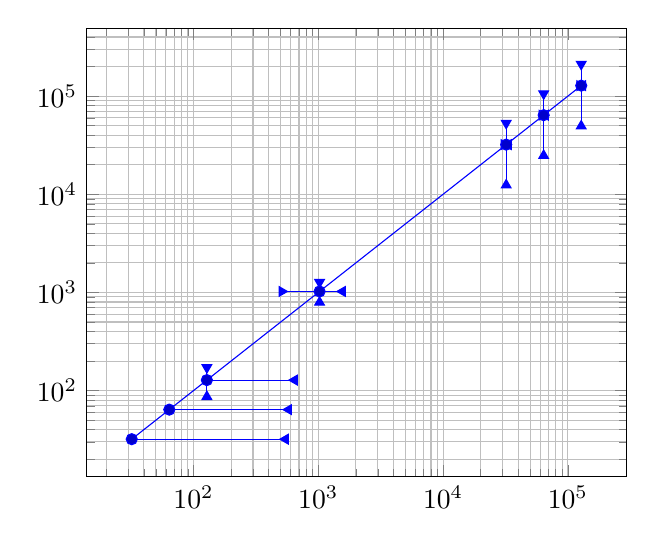
\begin{tikzpicture}
\begin{loglogaxis}[
	grid=both]
\addplot plot[
	error bars/.cd,
	y dir=both,y explicit relative,
	x dir=both,x fixed=500,
	error mark=triangle*,
]
	coordinates {
		(32,32)
		(64,64)
		(128,128) +- (0,0.3)
		(1024,1024) +- (0,0.2)
		(32068,32068)  +- (0,0.6)
		(64000,64000) +- (0,0.6)
		(128000,128000) +- (0,0.6)
	};

\end{loglogaxis}
\end{tikzpicture}

\testsubsubsection{with plot table}
\begin{tikzpicture}
\begin{loglogaxis}[title={dof versus Lmax, table~\ref{tbl:k}}]
\addplot plot[
	error bars/.cd,
	y dir=both,y explicit relative,
] table[x=dof,y=Lmax,y error=Lmax_relerror] {plotdata/pgfplotstest_plot};
\end{loglogaxis}
\end{tikzpicture}

\testsubsubsection{with plot table from macro}
\begin{tikzpicture}
\begin{loglogaxis}[title={dof versus Lmax, table~\ref{tbl:k}}]
\addplot plot[
	/pgfplots/error bars/.cd,
	y dir=both,y explicit relative,
] table[x=dof,y=Lmax,y error=Lmax_relerror] from \TABLEMACRO;
\end{loglogaxis}
\end{tikzpicture}

\testsubsubsection{with plot table absolute}
\begin{tikzpicture}
\begin{loglogaxis}[grid=both,title={dof versus L2, table~\ref{tbl:k}}]
\addplot plot[
	/pgfplots/error bars/.cd,
	y dir=both,y explicit,
] table[x=dof,y=L2,y error=L2_abserror] {plotdata/pgfplotstest_plot};
\end{loglogaxis}
\end{tikzpicture}
}
